% Pre-ambulo
\documentclass[a4paper, 12pt]{abnt}

\usepackage[brazil]{babel}
\usepackage[latin1]{inputenc}
\usepackage[T1]{fontenc}
\usepackage{dsfont}
\usepackage{amssymb,amsmath}
\usepackage{multirow}
\usepackage[alf]{abntcite}
\usepackage[pdftex]{color, graphicx}
\usepackage{colortbl}
\usepackage{url}
\usepackage{abnt-alf}
\usepackage{abntcite}	
\usepackage{algorithm}
\usepackage{algorithmic}
\usepackage{pdfpages}



\usepackage{listings}
\usepackage{xcolor}

\colorlet{punct}{red!60!black}
\definecolor{background}{HTML}{EEEEEE}
\definecolor{delim}{RGB}{20,105,176}
\colorlet{numb}{magenta!60!black}

\lstdefinelanguage{json}{
    basicstyle=\normalfont\ttfamily,
    numbers=left,
    numberstyle=\scriptsize,
    stepnumber=1,
    numbersep=8pt,
    showstringspaces=false,
    breaklines=true,
    frame=lines,
    backgroundcolor=\color{background},
    literate=
     *{0}{{{\color{numb}0}}}{1}
      {1}{{{\color{numb}1}}}{1}
      {2}{{{\color{numb}2}}}{1}
      {3}{{{\color{numb}3}}}{1}
      {4}{{{\color{numb}4}}}{1}
      {5}{{{\color{numb}5}}}{1}
      {6}{{{\color{numb}6}}}{1}
      {7}{{{\color{numb}7}}}{1}
      {8}{{{\color{numb}8}}}{1}
      {9}{{{\color{numb}9}}}{1}
      {:}{{{\color{punct}{:}}}}{1}
      {,}{{{\color{punct}{,}}}}{1}
      {\{}{{{\color{delim}{\{}}}}{1}
      {\}}{{{\color{delim}{\}}}}}{1}
      {[}{{{\color{delim}{[}}}}{1}
      {]}{{{\color{delim}{]}}}}{1},
}


\usepackage{listings}
\usepackage{color}

\definecolor{dkgreen}{rgb}{0,0.6,0}
\definecolor{gray}{rgb}{0.5,0.5,0.5}
\definecolor{mauve}{rgb}{0.58,0,0.82}

\lstset{frame=tb,
  language=Java,
  aboveskip=3mm,
  belowskip=3mm,
  showstringspaces=false,
  columns=flexible,
  basicstyle={\small\ttfamily},
  numbers=none,
  numberstyle=\tiny\color{gray},
  keywordstyle=\color{blue},
  commentstyle=\color{dkgreen},
  stringstyle=\color{mauve},
  breaklines=true,
  breakatwhitespace=true,
  tabsize=3
}



%\usepackage{alg}
%\usepackage{hyperref}


% Redefinicao de instrucoes
\floatname{algorithm}{Algoritmo}
\renewcommand{\algorithmicrequire}{\textbf{Entrada:}}
\renewcommand{\algorithmicensure}{\textbf{Sa�da:}}
\renewcommand{\algorithmicend}{\textbf{fim}}
\renewcommand{\algorithmicif}{\textbf{se}}
\renewcommand{\algorithmicthen}{\textbf{ent�o}}
\renewcommand{\algorithmicelse}{\textbf{sen�o}}
\renewcommand{\algorithmicfor}{\textbf{para}}
\renewcommand{\algorithmicforall}{\textbf{para todo}}
\renewcommand{\algorithmicdo}{\textbf{fa�a}}
\renewcommand{\algorithmicwhile}{\textbf{enquanto}}
\renewcommand{\algorithmicloop}{\textbf{loop}}
\renewcommand{\algorithmicrepeat}{\textbf{repetir}}
\renewcommand{\algorithmicuntil}{\textbf{at� que}}
\renewcommand{\algorithmiccomment}[1]{\% #1}


% Definicao da lista de simbolos
% \simb[entrada na lista de simbolos]{simbolo}:
% Escreve o simbolo no texto e uma entrada na lista de simbolos.
% Se o parametro opcional e omitido, usa-se o parametro obrigatorio.
\newcommand{\simb}[2][]
{%
	\ifthenelse{\equal{#1}{}}
	{\addcontentsline{los}{simbolo}{#2}}
	{\addcontentsline{los}{simbolo}{#1}}#2
}
% Para aceitar comandos com @ (at) no nome
\makeatletter 
% \listadesimbolos: comando que imprime a lista de simbolos
\newcommand{\listadesimbolos}
{
	\pretextualchapter{Lista de s�mbolos}
	{\setlength{\parindent}{0cm}
	\@starttoc{los}}
}
% Como a entrada sera impressa
\newcommand\l@simbolo[2]{\par #1}
\makeatother


% Definicao da lista de abreviaturas e siglas
% \abrv[entrada na lista de simbolos]{abreviatura}:
% Escreve a sigla/abreviatura no texto e uma entrada na lista de abreviaturas e siglas.
% Se o parametro opcional e omitido, usa-se o parametro obrigatorio.
\newcommand{\abrv}[2][]
{%
	\ifthenelse{\equal{#1}{}}
	{\addcontentsline{loab}{abreviatura}{#2}}
	{\addcontentsline{loab}{abreviatura}{#1}}#2
}

% Para aceitar comandos com @ (at) no nome
\makeatletter 
% \listadeabreviaturas: comando que imprime a lista de abreviaturas e siglas
\newcommand{\listadeabreviaturas}
{
	\pretextualchapter{List of Acronyms} 
	% \setlength{\parindent}{0cm}
	ACID - Atomicity, Consistency, Isolation, Durability \\
	API - Application Programming Interface \\
	CAAS - Communication as a Service \\
	CMS - Content Management System \\
	CPU - Central Processing Unit \\
	CRUD - Create Retrieve Update Delete operation \\
	DB - Database \\
	DBAAS - Database as a service \\
	DBMS - Database Management System \\
	FTS - Full-Text Search \\
	GB - Gigabyte \\
	HTTP - Hypertext Transfer Protocol \\
	IAAS - Infrastructure as a Service \\
	IAAS - Infrastructure as a service \\
	IT - Information Technology \\
	ITIL - Information Technology Infrastructure Library \\
	JAR - Java Archive \\
	JDBC - Java Database Connectivity \\
	JSON - JavaScript Object Notation \\
	MAAS - Monitoring as a Service \\
	MVP - Minimum-Viable Product) \\
	NOSQL - New SQL (OR Not Only SQL) \\
	ORDB - Object Relational Database \\
	PAAS - Platform as a Service \\
	QOS - Quality of Service \\
	RDBMS - Relational Database \\
	REST - Representational State Transfer \\
	ROFR - Rate of faulty requests \\
	SAAS - Software as a Service \\
	SDK - Software development kit \\
	SLA - Service-Level Agreement \\
	SLO - Service-Level Objective \\
	SM - Systematic Mapping \\
	SOA - Service-oriented Architecture \\
	SQL - Standard Query Language \\
	TPC - , Transaction Processing Performance Council H Benchmark \\
	TTM - Time-to-market \\
	UDDI - Universal Description, Discovery, and Integration \\
	UI - User Interface \\
	WS - Web Service \\
	XAAS - Everything as a Service \\
	XML - Extensible Markup Language \\

}
% Como a entrada sera impressa
\newcommand\l@abreviatura[2]{\par #1}
\makeatother


% \listofalgorithms: comando que imprime a lista de algoritmos
\renewcommand{\listalgorithmname}{Lista de algoritmos}


% Hifeniza��o de palavras feita de forma incorreta pelo LaTeX
\hyphenation{PYTHON ou-tros}


% Inicio do documento
\begin{document}

	\frenchspacing
	
	% Capa (arquivo Includes/Capa.tex)
	% Capa
% Prote��o externa do trabalho e sobre a qual se imprimem as informa��es indispens�veis 
% � sua identifica��o.

% Especifica��o da capa
\begin{titlepage}
	\begin{center}
		
		% Cabe�alho (n�o deve ser modificado)
		% Cont�m o bras�o da Universidade, o logotipo do Departamento, al�m dos dados
		% relacionados � vincula��o do aluno (Universidade, Centro, Departamento e Curso)
		\begin{minipage}{2.3cm}
			\begin{center}
				
\includegraphics[width=2.25cm, height=2.68cm]{Imagens/Brasao-UFRN.jpg}
			\end{center}
		\end{minipage}
		\begin{minipage}{11.15cm}
			\begin{center}
				\begin{espacosimples}
					{\small \ \\
                       \textsc{Universidade Federal do Rio Grande do Norte}		   			\\
							  \textsc{Centro de Ci�ncias Exatas e da Terra}					\\
							  \textsc{Departmento de Inform�tica e Matem�tica Aplicada}	   	\\
							  \textsc{Programa de P�s-Gradua��o em Sistemas e Computa��o}  	\\
                       \textsc{Mestrado Acad�mico em Sistemas e Computa��o}}   				\\
				\end{espacosimples}
			\end{center}
		\end{minipage}
		\begin{minipage}{2.3cm}
			\begin{center}
				
\includegraphics[width=2.52cm, height=1.96cm]{Imagens/Logotipo-DIMAp.png}
			\end{center}
		\end{minipage}
			
		\vspace{6cm}
						
		% T�tulo do trabalho
		{\setlength{\baselineskip}%
		{1.3\baselineskip}
		{\LARGE \textbf{Guidelines for database transitioning on production environments}}\par}
			
		\vspace{3cm}
			
		% Nome do aluno (autor)
		{\large \textbf{Fabioea de Sousa Leal}}
						
		\vspace{6cm}
		
		% Local da institui��o onde o trabalho deve ser apresentado e ano de entrega do mesmo
		Natal-RN\\Julho de 2015
	\end{center}
\end{titlepage}

	% Folha de rosto (arquivo Includes/FolhaRosto.tex)
	% Folha de rosto
% Cont�m os elementos essenciais � identifica��o do trabalho.

% T�tulo, nome do aluno e respectivo orientador e filia��o
\titulo{\Large{Guidelines for database transitioning on production environments}}
\autor{Fabio de Sousa Leal}
\orientador[Orientador]{\par Martin A. Musicante}
\instituicao
{
	PPgSC -- Programa de P�s-Gradua��o em Sistemas e Computa��o\par 
	DIMAp -- Departamento de Inform�tica e Matem�tica Aplicada\par
   CCET -- Centro de Ci�ncias Exatas e da Terra\par
   UFRN -- Universidade Federal do Rio Grande do Norte
}
	
% Natureza do trabalho (n�o deve ser modificada)
\comentario
{
	Proposta de disserta��o de Mestrado  apresentada ao Programa de P�s-Gradua��o em Sistemas e Computa��o do Departamento de Inform�tica e Matem�tica Aplicada da Universidade Federal do Rio Grande do Norte como requisito parcial para a obten��o do grau de Mestre em Sistemas e Computa��o.\bigskip\\
   \textit{Linha de pesquisa}:\\Engenharia de Software
}
		
% Local e data
\local{Natal-RN}
\data{Julho - 2015}
	
\folhaderosto	
	
	% Folha de aprovacao (arquivo Includes/FolhaAprovacao.tex)
	% Folha de aprova��o
\begin{folhadeaprovacao}
	\setlength{\ABNTsignthickness}{0.4pt}
	\setlength{\ABNTsignwidth}{10cm}
	
	% Informa��es gerais acerca do trabalho 
	% (nome do autor, t�tulo, institui��o � qual � submetido e natureza)
	\noindent 
	Disserta��o de Mestrado sob o t�tulo \textit{Guidelines for database transitioning on production environments} apresentada por Nome completo do autor e aceita pelo Programa de P�s-Gradua��o em Sistemas e Computa��o do Departamento de Inform�tica e Matem�tica Aplicada da Universidade Federal do Rio Grande do Norte, sendo aprovada por todos os membros da banca examinadora abaixo especificada:
		
	% Membros da banca examinadora e respectivas filia��es
	\assinatura
	{
		Martin A. Musicante   			                  \\
		{\small Presidente}											          \smallskip\\ 
		{\footnotesize
			DIMAp -- Departamento de Inform�tica e Matem�tica Aplicada		   \\
		  	UFRN -- Universidade Federal do Rio Grande do Norte
		}
   }
      
   \assinatura
	{
      Marcia Jacyntha Nunes Rodrigues Lucena - Professora Adjunta 			                  \\
		{\small Examinador}											          \smallskip\\ 
		{\footnotesize
			DIMAp -- Departamento de Inform�tica e Matem�tica Aplicada		   \\
		  	UFRN -- Universidade Federal do Rio Grande do Norte
		}
   }   
   
   \assinatura
	{
      Tha�s Vasconcelos Batista - Professora Adjunta   			                  \\
		{\small Examinador}											          \smallskip\\ 
		{\footnotesize
			DIMAp -- Departamento de Inform�tica e Matem�tica Aplicada		   \\
		  	UFRN -- Universidade Federal do Rio Grande do Norte
		}
	}
		
	\vfill
	
	\begin{center}
		Natal-RN, data da defesa (dia, m�s e ano).
	\end{center}
\end{folhadeaprovacao}
	
	
	% Dedicatoria (arquivo Includes/Dedicatoria.tex)
	% Dedicat�ria

\chapter*{}
\vspace{15cm}
\begin{flushright}
	Homenagem que o autor presta a uma ou mais pessoas.
\end{flushright}
	
	% Agradecimentos (arquivo Includes/Agradecimentos.tex)
	% Agradecimentos

\chapter*{Agradecimentos}

Agradecimentos dirigidos �queles que contribu�ram de maneira relevante � elabora��o do trabalho, sejam eles pessoas ou mesmo organiza��es.
   
   % Epigrafe (arquivo Includes/Epigrafe.tex)
	% Ep�grafe (cita��o seguida de indica��o de autoria)

\chapter*{}
\vspace{15cm}
\begin{flushright}
	\textit
	{
		Cita��o
	}\medskip\\ 
	Autor
\end{flushright}
	
	% Resumo em l�ngua vernacula (arquivo Includes/Resumo.tex)
	% % Resumo em l�ngua vern�cula
\begin{center}
	{\Large{\textbf{Using SLA to guide software migration to the cloud: An empirical study}}}
\end{center}

\vspace{1cm}

\begin{flushright}
	Autor: Fabio de Sousa Leal\\
	Orientador: Martin A. Musicante
\end{flushright}

\vspace{1cm}

\begin{center}
	\Large{\textsc{\textbf{Resumo}}}
\end{center}

\noindent O resumo deve apresentar de forma concisa os pontos relevantes de um texto, fornecendo uma vis�o r�pida e clara do conte�do e das conclus�es do trabalho. O texto, redigido na forma impessoal do verbo, � constitu�do de uma seq��ncia de frases concisas e objetivas e n�o de uma simples enumera��o de t�picos, n�o ultrapassando 500 palavras, seguido, logo abaixo, das palavras representativas do conte�do do trabalho, isto �, palavras-chave e/ou descritores. Por fim, deve-se evitar, na reda��o do resumo, o uso de par�grafos (em geral resumos s�o escritos em par�grafo �nico), bem como de f�rmulas, equa��es, diagramas e s�mbolos, optando-se, quando necess�rio, pela transcri��o na forma extensa, al�m de n�o incluir cita��es bibliogr�ficas.

\noindent\textit{Palavras-chave}: Palavra-chave 1, Palavra-chave 2, Palavra-chave 3.
	
	% Abstract, resumo em l�ngua estrangeira (arquivo Include/Abstract.tex)
	% Resumo em l�ngua estrangeira (em ingl�s Abstract, em espanhol Resumen, em franc�s R�sum�)
\begin{center}
	{\Large{\textbf{TODO::CHANGE::Guidelines for database transitioning on production environments}}}
\end{center}

\vspace{1cm}

\begin{flushright}
	Author: Fabio de Sousa Leal\\
	Supervisor: Martin A. Musicante
\end{flushright}

\vspace{1cm}

\begin{center}
	\Large{\textsc{\textbf{Abstract}}}
\end{center}

\noindent Component-based Software Engineering (CBSE) and Service-Oriented Architecture (SOA) became  popular ways to develop software over the last years. During the life-cycle of a software, several components and services can be developed, evolved and replaced. In production environments, the replacement of core components, such as databases, is often a risky and delicate operation, where several factors and stakeholders take place.

Service Level Agreements (SLA), according to ITILv3's official glossary, is ``an agreement between an IT service provider and a customer. The agreement consists on a set of measurable constraints that a service provider must guarantee to its customers.''. In practical terms, it is a document that a service provider delivers to its consumers with minimum quality of service (QoS) metrics.

This work assesses and improves the use of SLAs to guide the transitioning process of databases on production environments. In particular, in this work we propose SLA-Based Guidelines/Process to support migrations from a relational database management system (RDBMS) to NoSQL one. Our study is validated by case studies.

\noindent\textit{Keywords}: SLA, Database, Migration.
	
	% Lista de figuras
	\listoffigures

	% Lista de tabelas
	% \listoftables
	
	% Lista de abreviaturas e siglas
	\listadeabreviaturas
	
	% Lista de s�mbolos
	% \listadesimbolos
	
	% Lista de algoritmos (se houver)
	% Devem ser inclu�dos os pacotes algorithm e algorithmic
	% \listofalgorithms
	
	% Sum�rio
	\sumario

	% Parte central do trabalho, englobando os cap�tulos que constituem o mesmo
	% Os referidos cap�tulos devem ser organizados dentro do diret�rio "Cap�tulos"

	% Capitulo 1: Introdu��o (arquivo Includes/Introducao.tex)
	% Introdu��o
\chapter{Introduction}

The goal of this chapter is to present the technical concepts for a better understanding of our job. 


\section{Cloud Computing \& The technological shift}

The adoption of cloud solutions is growing fast among organizations~\cite{6546068}.
Centralized (mostly mainframe) technology is being replaced by distributed and more flexible forms of data storage and processing.
This change of paradigm is motivated by the necessity to improve the use of resources, as well as by the increasing velocity in which data is produced.

In this scenario, transitions must take into account the quality of the service delivered by the new solutions.

On the early 90's it was commonplace for every Information Technology (IT) company to have its own Data Center with huge servers and mainframes. 
IT costs were high, and high-performance computing was available only for big companies, as data centers required a large physical infrastructure and have high costs for maintenance~\cite{Armbrust09m.:above}.

The regular way of building a web application was to use a client-server approach, where the server was a powerful (and expensive) machine. 
At the same time, new players, such as Google or Yahoo, were rising with bigger missions: \textit{``to organize the world's information and make it universally accessible and useful''}~\cite{Spector:2012:GHA:2209249.2209262}. 
The popularization of the internet use incentivized new ways of commerce exchange, yielding an explosion in the amount of data produced and exchanged. 
It was \textit{just} impossible to store the petabytes of daily-generated data in a single server. 

From this point on, the community realized the economical convenience of building and maintaining several low-performance servers, instead of a single high-performance one, even if this this requires a change of culture in the administration of the new datacentres.
The new approach is also incompatible with the traditional way of building applications, that usually were designed to work on a single server and database. 

Several research initiatives were conducted in this area and a common solution was rising: to distribute data storage and processing. 
Google, Yahoo and other big IT players helped to build open source tools to make this approach possible, like Hadoop~\cite{5496972}.

This revolution brought to life the notion of \textit{Cloud Computing}, together with new concepts, such as Infrastructure as a Service \textit{(IAAS)}, Platform as a Service \textit{(PAAS)} and Software as a Service \textit{(SAAS)}~\cite{AViewOfCloudComputing}.
According to~\cite{AViewOfCloudComputing}, \textit{Cloud computing refers to both the applications delivered as services over the Internet and the hardware and systems software in the data centers that provide those services.} 


\section{Data Integration \& Polyglot Persistence}
On the last years, the number of Data Base (DB) Engines grew like never before~\cite{dbranking}. 
Along with the NoSQL (Not only SQL) movement and expansion of Social Networks, new concepts for Database Models appeared, like Document Store, Search Engines, Key-Value store, Wide Column Store, Multi-Model and Graph DBMS. 
In~\cite{dbranking} a ranking of the most popular DB engines is presented.

Today, instead of having a single Relational Database Management System (DBMS) for the whole application, it is efficient and cost-effective to have several Data Base Engines, one for each type of data that the application handles. 
This concept is called \textit{Polyglot Persistence}~\cite{sadalage2012nosql}.

As \cite{AdressingDataManagementCloud} illustrates, polyglot persistence is very useful in the context of  e-commerce applications that deal with a catalog, user access logs, financial information, shopping carts and purchase transactions, for example.
The notion of polyglot persistence is built upon the observation that the \textit{nature} of each data type is significantly different (i.e: user logs imply high volume of writes on multiple nodes, shopping carts need high availability and user sessions require rapid access for reads and writes). 

As computing services started to decentralize, developers started to build applications that depended of several data-sources. 
By this time the use of Web Services and Service Oriented Architecture (SOA) became more popular~\cite{Armbrust09m.:above}. 


\section{Systematic Mappings}
According to \cite{Petersen:2008:SMS:2227115.2227123}, ``\textit{A software engineering systematic map is a defined method to build a classification scheme and structure a software engineering field of interest.}''
Systematic Mapping studies provide a global view of a given research field and identify the quantity, results, and the kinds of researches in this field.

A Systematic map is composed by a number of steps (Figure~\ref{fig:sms}).
\begin{figure}[ht!]
\centering
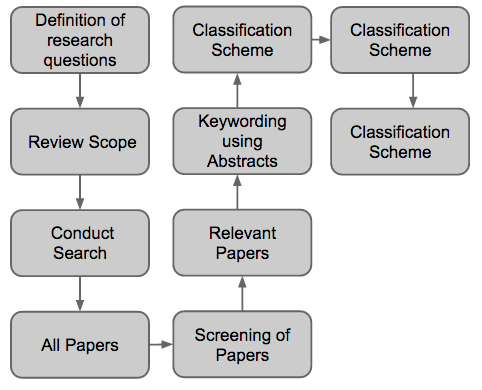
\includegraphics[width=100mm]{Imagens/pic1.png}
\caption{Systematic Mapping Steps~\cite{Petersen:2008:SMS:2227115.2227123}.\label{fig:sms}}
\end{figure}

On the first step, ``Definition of Research question'', the questions that must be answered on the survey are defined. 
On the ``Review Scope'' step, researchers target the papers/journal sources that will be taken into consideration on the systematic map. 
After that, the ``Search'' step is done using a set of predefined search engines and a body of papers (``All papers'') is retrieved. 

After an initial ``Screening of the papers'', the ``Relevant papers'' are chosen according to inclusion and exclusion criteria defined by the research team. 
At this point, the papers that will participate of the study are selected. 
The selection is based on the title, abstracts and keywords of each paper (``Keywording using Abstracts'').

After that, a ``Classification Scheme'' is built, defining different points-of-view (or facets) from which the body of papers will be classified. 
After matching each paper with the classification schema (``Data Extraction and Mapping Process''), the  systematic mapping is performed.
In this phase the relationships between the collected data (in the light of the classification scheme) are used to answer the research questions.


\section{Service Level Agreements (SLAs)}
According to \textit{ITILv3's} official glossary \cite{itilv3glossary}, a Service Level Agreement (SLA) is ``\textit{an agreement between an IT service provider and a customer. 
A service level agreement describes the IT service, documents service level targets, and specifies the responsibilities of the IT service provider and the customer.}'' 

The agreement consists on a set of measurable constraints that a service provider must guarantee to its customers.
In practical terms, it is a document that a service provider delivers to its consumers with minimum quality of service (QoS) metrics. 
If the service is delivered with a lower QoS than is promised on the SLA, consumers may be refunded or earn benefits that were accorded beforehand.    
	
	% Capitulo 1: Introdu��o (arquivo Includes/Introducao.tex)
	\chapter{Bibliographic Review}\label{bibreviewChap}

The goal of this chapter is to explore the main concepts that are related to our work. We begin by presenting popular concepts, such as Cloud Computing, \textit{Everything as a Service} strategy, NoSQL and Service Level Agreements. 
We also explain how each of these concepts are linked with this work.

\section{Cloud Computing}

Technology evolved with big steps over the last decades. Internet is now a pervasive concept and individuals can be connected virtually everywhere on Earth. \cite{Armbrust09m.:above}

Web applications and IT-based processes followed this evolution and today a number of companies rely on software on its production chain. Information Technology can be a competitive advantage of a company, but it \textbf{might not}  be part of its core business \cite{powell1997information}. In fact, this is a common scenario on a number of successful companies of the current century, as we might notice.

To avoid losing track of its core business, a number of companies now prefer to outsource (part of) their IT department to other companies \cite{quinn2013technology}. In other words, today it is possible to outsource IT infrastructure, product development and even the entire IT department to other companies.

In the late 60's, former Stanford University professor John McCarthy introduced the concept of time-sharing of computing services in a famous speech on time-sharing systems, as referenced by \cite{brendon} and \cite{wiki:mccarthy}. In fact, Prof. McCarthy believed that computer resources would be provided as commodities, like water and electricity.

Several years later, this concept brought to life the notion of \textit{Cloud Computing}, together with new concepts, such as Infrastructure as a Service \textit{(IAAS)}, Platform as a Service \textit{(PAAS)}, Software as a Service \textit{(SAAS)} and Everything as a Service \textit{(XaaS)}~\cite{AViewOfCloudComputing}.

According to~\cite{AViewOfCloudComputing}, \textit{Cloud computing refers to both the applications delivered as services over the Internet and the hardware and systems software in the data centers that provide those services.} 

\cite{stanoevskaslabeva2009grid} outlines some of the features of Cloud Computing:

\begin{itemize}
   \item{Cloud Computing is a new computing paradigm.}
   \item{The main features of clouds are virtualization and scalability on demand.}

   \item{Infrastructure resources (hardware, storage and system software) and applications
        are provided in X-as-a-Service manner.}
   \item{Utility computing and SaaS are delivered in an integrated manner. Computing might be consumed separately.}
   \item{Cloud services are consumed either via Web browser or via a defined API.}
\end{itemize}


The ``pay as you go'' model offered by Cloud providers revolutionized the IT market, enabling companies to consume computing resources that matched its needs. Small companies became more competitive, as there is no more need to build datacentres to scale companies. As professor McCarthy believed, computing resources can now be seen as commodities for a company, just like water and electricity.  

\section{Everything as a Service - XaaS}

Service-Oriented Architecture (SOA) defines several concepts of ``as-a-service'' models. To enumerate a few, it is possible to find mentions to Platform as a Service (PaaS), Infrastructure as a Service (IaaS), Software as a Service (SaaS), Database as a Service (DBaaS), Desktop as a Service (DaaS), Monitoring as a Service (MaaS) and Communication as a Service (CaaS) on the literature. 

To summarize all these concepts, a new term arose: Everything as a service (XaaS)\cite{7214098}\cite{Armbrust09m.:above}.

On the context of Cloud Computing, however, three of these concepts are the most relevant, and we define them more precisely:

\begin{itemize}
   \item{Infrastructure as a service (IaaS): It is the most simple kind of ``as-a-service'' product and is located on the base of the IaaS-PaaS-SaaS Stack (Figure \ref{fig:cloudstach}). IaaS mostly refers to (Virtual) Machines, Storage Devices, Network Infrastructure and other infrastructural services that are available on Cloud Computing vendors.} Some examples of IaaS providers are \cite{amazonec2} \cite{rackspace} and \cite{azure}. 
   \item{Platform as a Service (PaaS): PaaS refers to the development environments that are available from cloud vendors. PaaSs are composed by a development stack, and generally offer databases, web servers and execution runtime. Examples of PaaSs are \cite{beanstalk}, \cite{azure} and \cite{GAE}.  }
   \item{Software as a Service (SaaS): Software as a Service refers to the applications that run on the cloud: Webmail, CRM, Gaming Platforms, Learning Management Systems, etc. SaaSs, just as IaaSs and PaaSs, generally charge its users a periodic fee. The fee is generally conceived in a pay-as-you-go model, so users get charged in a scalable way.  
}

\end{itemize}



\begin{figure}[ht!]
\centering
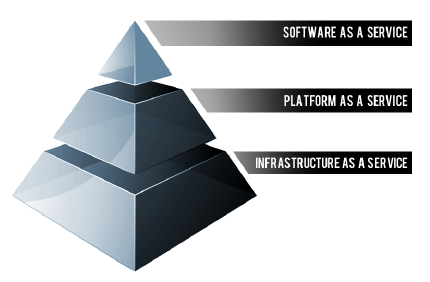
\includegraphics[width=80mm]{cloud_stack.png}
\caption{IaaS-PaaS-SaaS Stack~\cite{kepes2011understanding}.\label{fig:cloudstach}}
\end{figure}

Since the beginning of the Cloud movement several discussions were held concerning the security of Clouds. \cite{2010security} discusses that the security threats that arise on Cloud Computing are the result of users/enterprise lack of control of the IaaS layer. Not all companies know where their documents/data is physically stored and what are the security instruments that must be used to assure data safety on Cloud environments.

On the base of the pyramid of Figure~\ref{fig:cloudstach} is located the IaaS - machines, Network Infrastructure and other Simple Services. Above IaaS lies the PaaS layer - It acts as a ``middleware'' between the SaaS Layer and the IaaS layer, providing the development environments that developers need to deploy applications. On the top of the image is located the SaaS layer. 

To have a better understanding of the security concerns on Cloud Computing, a deeper understanding of its architecture is needed. Figure~\ref{fig:cloudmodel} illustrates the reference model for cloud computing \cite{alliance2009}.

The IaaS layer is generally composed by five elements: API's, Abstraction, Core Connectivity, Hardware and Facilities. A cloud provider may be vulnerable if a security breach is discovered on its APIs or Abstraction Layer, for example. Another possible vulnerability in cloud providers are outages. In 2014, major cloud providers, such as \cite{amazonec2}, \cite{azure}, \cite{rackspace} and \cite{GAE} experienced downtime \cite{cloudoutageaudit}.

Similar security issues can be found on the PaaS and SaaS layers.

\begin{figure}[ht!]
\centering
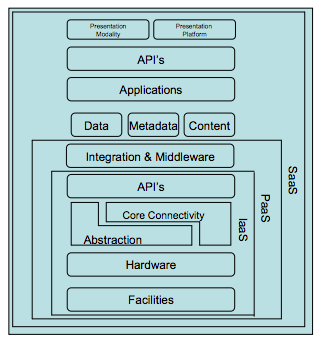
\includegraphics[width=80mm]{Imagens/cloudreferencemodel.png}
\caption{Cloud Reference Model ~\cite{alliance2009}.\label{fig:cloudmodel}}
\end{figure}


\section{The technological shift}
The adoption of cloud solutions is growing fast among organizations~\cite{Armbrust09m.:above}.
Centralized (mostly mainframe) technology is being replaced by distributed and more flexible forms of data storage and processing.
This change of paradigm is motivated by the necessity to improve the use of resources, as well as by the increasing velocity in which data is produced.

On the early 90's it was commonplace for every Information Technology (IT) company to have its own Data Center with huge servers and mainframes. 
IT costs were high, and high-performance computing was available only for big companies, as data centers required a large physical infrastructure and have high costs for maintenance~\cite{Armbrust09m.:above}.

The regular way of building a web application was to use a client-server approach, where the server was a powerful (and expensive) machine. 
At the same time, new players, such as Google or Yahoo, were rising with bigger missions: \textit{``to organize the world's information and make it universally accessible and useful''}~\cite{Spector:2012:GHA:2209249.2209262}. 
The popularization of the internet use incentivized new ways of commerce exchange, yielding an explosion in the amount of data produced and exchanged. 
It was \textit{just} impossible to store the petabytes of daily-generated data in a single server. 

From this point on, the community realized the economical convenience of building and maintaining several low-performance servers, instead of a single high-performance one, even if this this requires a change of culture in the administration of the new datacentres. The new approach (scale-out) is also incompatible with the traditional way of building applications (scale-up), that usually were designed to work on a single server and database. Both approaches are represented on Figure~\ref{fig:scaleupout}.

\begin{figure}[ht!]
\centering
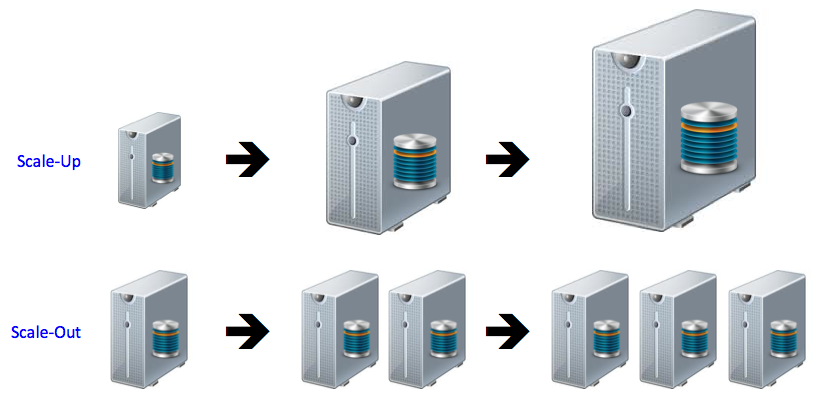
\includegraphics[width=100mm]{scaleOut.png}
\caption{Scale Out vs Scale Up.\cite{scaleupref} \label{fig:scaleupout}}
\end{figure}


Several research initiatives were conducted in this area and a common solution was rising: to distribute data storage and processing. 
Google, Yahoo and other big IT players helped to build open source tools to make this approach possible, like Hadoop~\cite{5496972}.



\section{Data Integration, NoSQL Movement \& Polyglot Persistence}

Along with the NoSQL (Not only SQL) movement and expansion of Social Networks, new concepts for Database Models became popular, like Document Store, Search Engines, Key-Value store, Wide Column Store, Multi-Model and Graph DBMS \cite{dbrankingchart}. 

New ways to store and retrieve data are in high demand, as Figure~\ref{fig:popularityDB} suggests. This chart shows trends of popularity growth among categories. As \cite{dbrankingchart} explains: \textit{``In order to allow comparisons, the initial value is normalized to 100. For most of the categories the trend starts with January 2013 but search engines and multivalue DBMS are only collected since February 2013 and May 2013.''}. 



\begin{figure}[ht!]
\centering
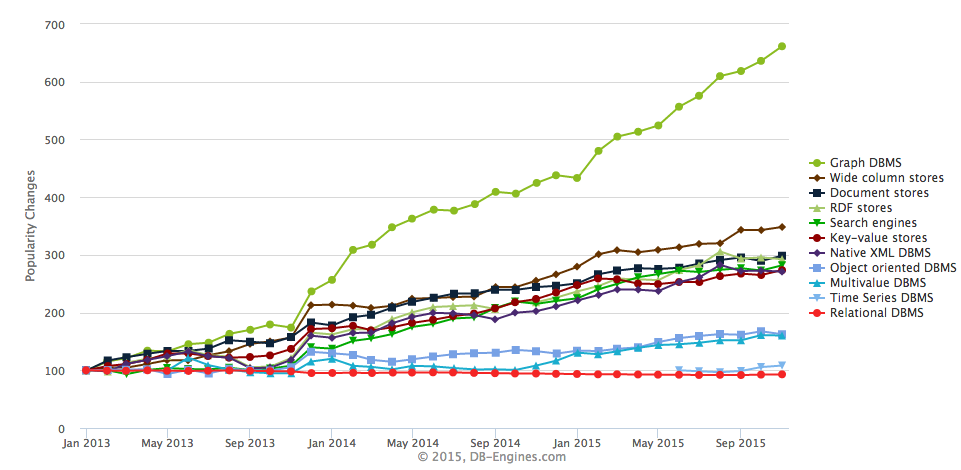
\includegraphics[width=150mm]{popularityDB.png}
\caption{Database Popularity Growth Chart \cite{dbrankingchart}.\label{fig:popularityDB}}
\end{figure}

Figure \ref{fig:currentPopularity} presents the current database popularity by categories. It shows that despite of the NoSQL movement, relational databases are still responsible for more than 80\% of the databases used in applications.

\begin{figure}[ht!]
\centering
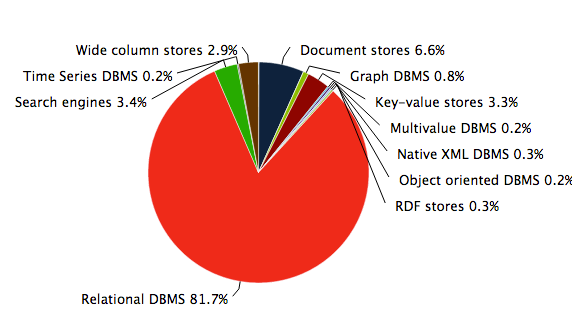
\includegraphics[width=100mm]{Imagens/DBpie.png}
\caption{Database Popularity Chart \cite{dbrankingchart}.\label{fig:currentPopularity}}
\end{figure}


Today, instead of having a single Relational Database Management System (DBMS) for the whole application, it is efficient and cost-effective to have several Data Base Engines, one for each type of data that the application handles. 
This concept is called \textit{Polyglot Persistence}~\cite{sadalage2012nosql}. In~\cite{dbranking} a ranking of the most popular DB engines is presented.

As \cite{AdressingDataManagementCloud} illustrates, polyglot persistence is very useful in the context of  e-commerce applications that deal with a catalog, user access logs, financial information, shopping carts and purchase transactions, for example.

The notion of polyglot persistence is built upon the observation that the \textit{nature} of each data type is significantly different (i.e: user logs imply high volume of writes on multiple nodes, shopping carts need high availability and user sessions require rapid access for reads and writes). 

As computing services started to decentralize, developers started to build applications that depended of several data-sources. 
By this time the use of Web Services and Service Oriented Architecture (SOA) became more popular~\cite{Armbrust09m.:above}. 



\section{Transitioning Processes}

In 1965 Gordon E. Moore, Intel's co-founder, published a paper stating that the number of components in integrated circuits had doubled every two years, and would continue to do so for the at least another decade \cite{658762}. Today, this statement is known as ``Moore's Law''.

A similar trend is stablished for commercial software. Wirth's law, Gates' law (Microsoft) or Page's law (Google) state that ``the speed of software halves every 18 months'', compensating Moore's law. \cite{wirth1995a}\cite{brinbreaking}

In other words, software components evolve in the opposite direction that hardware evolves. Useful software are usually versioned, updated and patched on a regular basis. As stated by \cite{922739}, maintaining software products is not cheap, and generally consumes on average 60\% of software costs.

Time-to-market (TTM) is the length of time that takes for from a product being conceived until its available for sale. Minimum-Viable-Product (MVP) is the product with the highest return on investment versus risk \cite{blank2013four}. Building a MVP and selling it should be the primary goal of a startup \cite{blank2013four}. 

The current economy demands faster shipping of software products in order to meet the desired TTM of software products and to deploy MVPs in less time. Cloud computing and Agile Methods made software development and deployment faster, cheaper and easier for a number of companies. 

One of the points of the 12 principles of the Agile Manifesto \cite{fowler2001agile} is \textit{``Deliver working software frequently, from a couple of weeks to a couple of months, with a preference to the shorter timescale''}.

This need for speed on software delivery has its downsides, however. Decisions must be made by the IT department on a short time schedule, sometimes leaving not enough time to make the best choices on the technologies that should be used on a software product. This and other factors often leads to a software migration, replacement or transitioning scenario. In this scenario (part of) a software is replaced with a more suitable alternative.

In the context of Service-Oriented Architecture this might be seen as the replacement of a Service. In a Multitier architecture scenario this might be seen as the replacement of an entire layer. In fact, basically any component of a \textbf{modular} software can be replaced, migrated or upgraded. 

Examples of Software migrations are numerous on the industry. To number a few: 
\begin{itemize}
\item{Spotify migrated their user base from Postgres to Cassandra\cite{spotifyEngineering}}
\item{Google moved from MySQL to MariaDB \cite{googleMariaDB}}
\item{Twitter moved from Ruby-On-Rails to Java \cite{twitterRails}}
\end{itemize}

Our work focuses specifically on Database Transitioning scenarios. We propose a set of guidelines to justify and guide the transitions from RDBMs to NoSQL databases;

\section{Systematic Mappings}
According to \cite{Petersen:2008:SMS:2227115.2227123}, ``\textit{A software engineering systematic map is a defined method to build a classification scheme and structure a software engineering field of interest.}''
Systematic Mapping studies provide a global view of a given research field and identify the quantity, results, and the kinds of researches in this field.

A Systematic mapping study is composed by a number of steps (Figure~\ref{fig:sms}).
\begin{figure}[ht!]
\centering
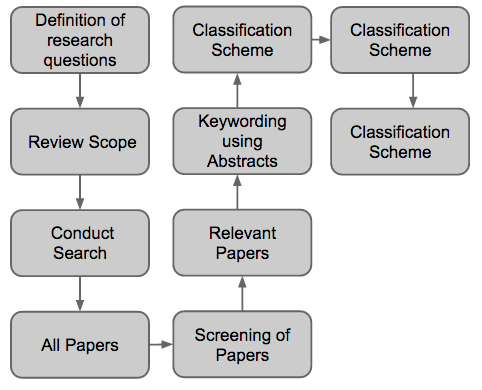
\includegraphics[width=100mm]{Imagens/pic1.png}
\caption{Systematic Mapping Steps~\cite{Petersen:2008:SMS:2227115.2227123}.\label{fig:sms}}
\end{figure}

On the first step, \textit{Definition of Research question}, the questions that must be answered on the survey are defined. 
On the \textit{Review Scope} step, researchers target the papers/journal sources that will be taken into consideration on the systematic map. 
After that, the \textit{Search} step is done using a set of predefined search engines and a body of papers (\textit{All papers}) is retrieved. 

After an initial \textit{Screening of the papers}, the \textit{Relevant papers} are chosen according to inclusion and exclusion criteria defined by the research team. 
At this point, the papers that will participate of the study are selected. 
The selection is based on the title, abstracts and keywords of each paper (\textit{Keywording using Abstracts}).

After that, a \textit{Classification Scheme} is built, defining different points-of-view (or facets) from which the body of papers will be classified. 
After matching each paper with the classification schema (\textit{Data Extraction and Mapping Process}), the  systematic mapping is performed.
In this phase the relationships between the collected data (in the light of the classification scheme) are used to answer the research questions.

In \cite{fabioMartinSM} a Systematic mapping study was developed to investigate the use of Service-Level-Agreements (SLAs) on database-transitioning scenarios and to verify how SLAs can be used in this processes. The results of this study are presented in Section \ref{oursystematicmapping}.

\section{Service Level Agreements (SLAs)}

In the field of Law, a contract (or agreement) is generally a written document concerning any point of interest between two parties, each of whom intends to create legal obligations between them. In business environments, contracts are highly necessary to avoid unpleasant situations between a provider and a consumer. 

In the context of service provisioning, it is common to refer to contracts (or agreements) as ``Service-Level agreements'' (SLA's), as the name suggests.  

According to \textit{ITILv3's} official glossary \cite{itilv3glossary}, a Service Level Agreement (SLA) is ``\textit{an agreement between an IT service provider and a customer. 
A service level agreement describes the IT service, documents service level targets, and specifies the responsibilities of the IT service provider and the customer.}'' 

The agreement consists on a set of measurable constraints that a service provider must guarantee to its customers.
In practical terms, it is a document that a service provider delivers to its consumers with minimum quality of service (QoS) metrics. 
If the service is delivered with a lower QoS than is promised on the SLA, consumers may be refunded or earn benefits that were accorded beforehand. 

In the next subsection we present the life-cycle of an SLA, explaining in details each step of it. 

\subsection{The Life-Cycle of an SLA}

The Life-cycle of an SLA consists on six steps, as presented on Figure~\ref{fig:sla-lifecycle}. Each step is explained in the following subsections. 

\begin{figure}[ht!]
\centering
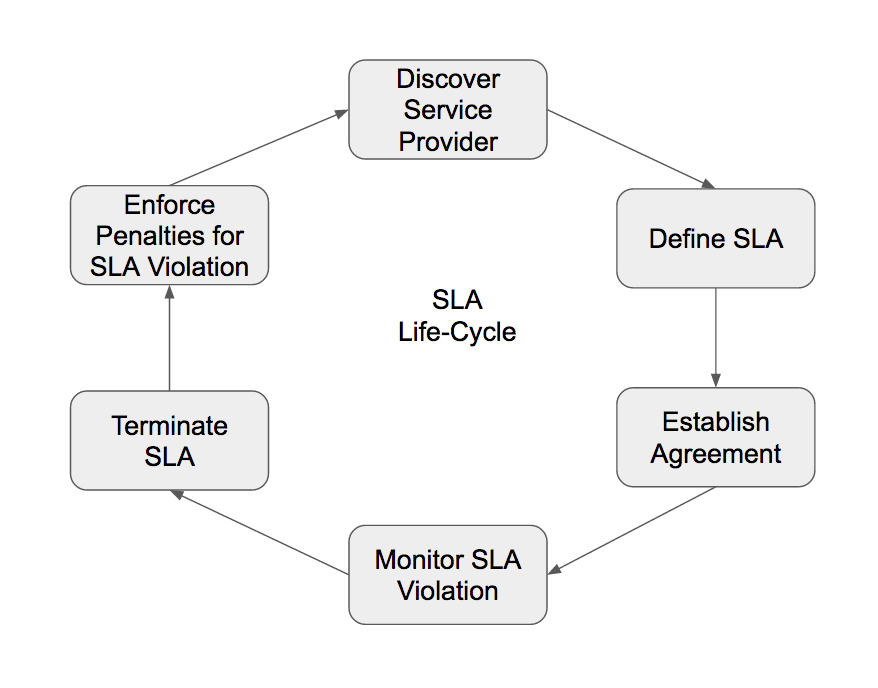
\includegraphics[width=90mm]{Imagens/sla-lifecycle.png}
\caption{SLA Life-cycle \cite{wu2012service}}.\label{fig:sla-lifecycle}
\end{figure}

\subsubsection{Discover Service Provider}
On the first step \textit{(Discover Service Provider)}, a consumer tipically discovers several service providers that may fulfill its needs on a specific scenario. On the domain of Web Services, \textit{Universal Description, Discovery, and Integration} (UDDI) can be used to retrieve a list of web services that might be used to achieve a goal, for example. 

In a Cloud Computing scenario, it is possible to buy computing services from a number of providers, and a cloud-service broker could be used to retrieve a list of available providers. This scenario is very common in cloud computing auctions \cite{7145493}, a new concept that arised with cloud computing and was made possible by companies like Hetzner.com, a company that hosts regular auctions of its computing resources.


\subsubsection{Define SLA}
The second step of the SLA life-cycle \textit{(To Define SLA)} is when an SLA is proposed by the provider. Several works, such as \cite{6846456} and \cite{kouki:hal-00675077} address the issue of specifying an SLA. WS-Agreement \cite{citeulike:2805191} and WSLA \cite{4578560} are very important works on this area. As it is presented on \cite{fabioMartinSM}, there are several ways to specify SLA, but none of them are considered a de-facto standard. 

\cite{fabioMartinSM} also shows that there are several ways to represent an SLA. To enumarate a few, it is possible to represent an SLA as a \textit{i) a natural-language document}, and \textit{ii) an ontology} \textit{automated test suite (unit tests, integration tests)}.

\subsubsection{Establish Agreement}

As stated on the beginning of this secttion, an SLA is a contract between a provider and a consumer. The points of interest of this contract are known as \textit{Service-Level Objectives} (SLOs).

According to \cite{sturm2000foundations}, SLOs must respect a series of features. They must be \textit{Attainable},  \textit{Repeatable},  \textit{Measurable},  \textit{Understandable},  \textit{Meaningful},  \textit{Controllable},  \textit{Affordable} and \textit{Mutually acceptable}. 

Each SLA may explicitly define the ``hardness'' of its SLOs in terms of time. In other words, an SLA can specify what is the fault tolerance rate of each of its SLOs. 

An example can be given to clarify this concept: Two telecommunication companies may have different SLAs regarding the uptime of their services given a fixed period of time. \textbf{Company A} may assure that their uptime is 99.9\% of the time under the period of a year, and \textbf{Company B} may assure that their uptime is 99.99\%. 

In this scenario, it is said that the SLA of Company B is ``harder'' than the SLA of Company A. Figure~\ref{fig:sla-agreement} compares the Availability SLO defined in SLAs of some popular cloud services.

\begin{figure}[ht!]
\centering
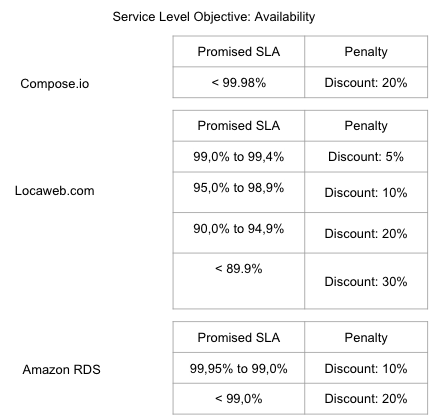
\includegraphics[width=120mm]{slo-cloudServices.png}
\caption{Service Level Objective: Availability on Cloud Services \cite{locawebsla}\cite{composesla}\cite{amazonrdssla}}\label{fig:sla-agreement}
\end{figure}

After chosing the service and defining the SLOs, SLA might be established between a consumer and the provider - the third step of th SLA life-cycle. 

\subsubsection{Monitor SLA violation}
The fourth step \textit{(Monitor SLA violation)} is one of the most important on the SLA life-cycle. It is in this step where the consumer protects himself against unfulfilled SLOs. 

Several frameworks and processes might be used to measure and monitor SLA violation. As SLAs do not present a standard way for representation, it is also difficult to find a standardized way to monitor SLA violation. 

\cite{ranna2008} presents three ``monitoring-models'' for SLA violation: 

\begin{itemize}
   \item{\textit{All-or-nothing}: In a all-or-nothing situation, \textbf{all} the SLOs must be satisfied to guarantee that the SLA is still valid.}
   \item{\textit{Partial}: In a partial scenario, the SLA specifies what are the SLOs that may not be broken, and declares rules less important SLOs.}
   \item{\textit{Wheighted Partial}: In a wheighted partial scenario, the consumer and provider specify thresholds that must be met for specific SLOs. If the service quality drops below a threshold, a penalty can be applied. 
}

\end{itemize}

In the context of Web Apps it is also possible to monitor SLA violations with the help of web applications, such as \cite{datadog}, \cite{appsee} and \cite{newrelic}. These tools offer graphical dashboards and alerts when SLAs defined by the software team are violated. The tools are able to monitor the three layers of a web application: front-end, business logic and databases. AJAX calls, plugins and server daemons are used to monitor each part of the web stack. 

\subsubsection{Terminate SLA}
An important question of the life-cycle of a SLA (fith step) is \textit{when} the termination of an SLA is needed. If the termination is due to an SLA violation, it is important to know what party broke the SLA and what are the consequences for the parts.

These situations must be explicitly declared in the initial SLA to avoid unpleasant situations between the provider and the consumer in the future.

\subsubsection{Enforce Penalties for SLA violation}
The sixth step \textit{(Enforce penalties for SLA violation)} can be performed if the penalties that were previously defined are being hit in a regular basis or if both parties of the SLA agree. Several works, as \cite{Lee:2010:PSR:1844765.1845204} propose penalty models/processes for SLA violations. These processes can be analyzed and used by the SLA parties. 

\section{Our Systematic Mapping}\label{oursystematicmapping}

To provide us a better understanding over the use of SLAs in component / service migrations, we have performed a Systematic Mapping study to assess the use of SLAs in database transition scenarios, specifically on migrations from relational databases with NoSQL ones. 

This study is available on Appendix \ref{appendix}. 

\subsection{Identified problems}

As a result, we have analyzed over 70 publications closely related to the use of SLAs in migration scenarios. The study revealed a number of interesting outcomes, and we emphasize two of them below:

\begin{itemize}
\item{No publication was found addressing the problem of measuring the overall improvements after a database transition. Several benchmarking frameworks, such as TPC-H, TPC-DS and YCSB were identified \cite{6616442} during our survey, though. These benchmarking frameworks could be a good starting point to develop new tools and specialized frameworks to solve this problem and might be used in our study to validate that a migration was successful.
}

\item{ \cite{6253526}, \cite{6461875}, \cite{6511780} and \cite{Xiong:2011:APA:2038916.2038931} propose SLA-centric/User-Centric solutions to monitor the performance of web applications. All these solutions are technology-agnostic and could be used to monitor the performance improvements promised by a database transitioning process. Industry experts also pointed out that there are some services, such as New Relic~\cite{newrelic}, Appsee~\cite{appsee} and Datadog~\cite{datadog} that provide SLA-monitoring tools for web apps. 

The systematic mapping revealed no open source solution to monitor Application SLAs in a user-centered view (application level).  
}

\end{itemize}




	
	% Capitulo 2: Segundo cap�tulo (arquivo Includes/Capitulo2.tex)
	% Cap�tulo 2
\chapter{The Problem - Breakdown}\label{theProblemChap}

TODO: In this section we detail ...

\section{Problem Breakdown}
TODO: Breakdown each step of the problem.



\section{Proposed solution}

Service-Oriented Architecture (SOA) suggests that a Software Component can be seen as a set of sub-services. In the context of a Web Application, for example, it is possible to entirely replace a component just by changing the API address that it uses. This scenario of component replacement on cloud-based applications can be seen on (Figure~\ref{fig:apireplacement}).

\begin{figure}[ht!]
\centering
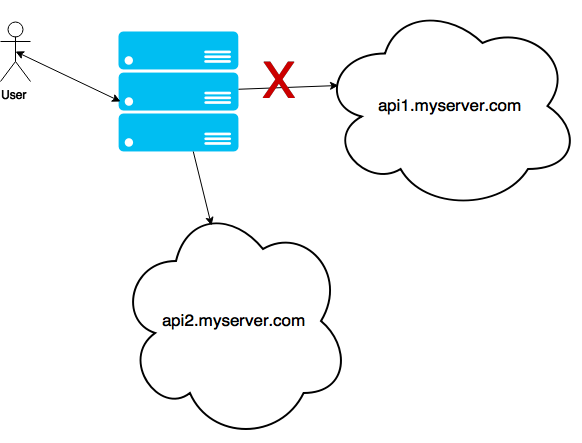
\includegraphics[width=100mm]{api.png}
\caption{Component replacement on cloud-based software.\label{fig:apireplacement}}
\end{figure}

As Section \ref{bibreviewChap} presents, contributions can be made in the context of proposing SLA-Based and user-centered solutions to monitor component replacement scenarios.

In this work we assess the use of a SLA-Guided process to support the migration/replacement of relational databases with NoSQL ones. This process was developed and assessed with case studies.

The boundaries of this work could then be broadened to support the conception of a SLA-Guided process to support the migration/replacement of sotware components based on the cloud in future works.


\section{Roadmap}
%Detalhar l� em cima o que � PDCA
%nosso estudo vai ser baseado no PDCA, detalhado l� em cima, e pode ser dividido em 6 fases principais: 

To provide a better understanding of our work, we splitted the research in six main phases:

\begin{table}[!htb]
   \textsf{\caption{Work Phases.}} \label{tab:WorkPhasesTable}
   \centering
   \medskip
      \begin{tabular}{ | p{1cm}| p{2.5cm} | p {8cm} |}
   \hline
   Phase & Title & Description  \\ \hline
   1 & Identification of Case Studies \& SLAs  & On this step we aim to identify examples where a Database transition is needed or recommended in order to satisfy a SLA.
   We will try to work on production-ready and open-source softwares. If the complexity of these projects is too large for our scope, we will design and develop our own scenarios. \\ \hline
   2 & Plan & After the scenarios have been identified, we will propose architectural changes that could satisfy the SLA. These changes will be proposed by literature reviews and survey of industry experts.\\ \hline
   3 & Do & On this step we implement the architecture proposed on the previous step. \\ \hline
   4 & Check & On the check step we will verify if the proposed architecture and implementation satisfies the SLAs identified on the first step. \\ \hline
   5 & Act & Tweaks can be needed on the proposed architecture and implementation if the SLA is still not satisfied by the changes made on the previous step. On the act phase we investigate what else can be done to satisfy the SLA and refine the process defined on step 2. \\ \hline
   6 & Final Results & On the final step we aim to publish the results of our work on relevant database-related conferences and workshops. \\ \hline
   
   \end{tabular}
\end{table}





Each of these phases is composed by a number of steps, described below:
\begin{enumerate}
\item{Phase 1 - Identification of Case Studies \& SLAs }
\begin{enumerate}
\item {Step 1.1 - Scenario identification / Implementation: On this step we will search for open source projects and real-world scenarios where a Relational Database bottleneck has been identified. If the scope of these scenarios become too large, we will implement our own scenarios; }
\item {Step 1.2 - Identification of broken SLAs: We need to identify that the a set a constraints (i.e: execution time of a query) is not being met by the current architecture;}
\item {Step 1.3 - Implementation of ``runnable SLAs'' : On this step we will implement executable versions of the SLA identified on the previous step. These ``runnable SLAs" will be used to verify that a set of constraints is not being met by the current architecture. }
\item {Step 1.4 - Execution reports: After an executable SLA has been identified and implemented, execution reports will be consolidated to prove that the constraints of the SLA are being broken by the current architecture of the scenario.}

\end{enumerate}


\item{Phase 2 - Plan}
\begin{enumerate}
\item{Step 2.1 - Literature Review for each scenario: We will evaluate and search for solutions on how each scenario can make use of a NoSQL Database to meet the desired SLA; }
\item{Step 2.2 - Survey of industry experts: We will survey industry experts on how they would propose a NoSQL architecture to solve the problem described on each scenario. }
\end{enumerate}

\item{Phase 3 - Do}
\begin{enumerate}
\item{Step 3.1 - Planning of changes: We will gather the results from the previous phase and design the changes that will be performed on each scenario;}
\item{Step 3.2 - Implementation: We will implement the changes identified on the previous step. }
\end{enumerate}

\item{Phase 4 - Check}
\begin{enumerate}
\item {Step 4.1 - New Execution Reports: The same SLAs identified on the first step will be run on the modified scenarios, and execution reports will be consolidated.}
\item {Step 4.2 - Comparison of Results: The reports extracted on steps 4.1 and 1.4 will be compared to check if the changes made on Phase 3 satisfied the proposed SLA.}
\end{enumerate}

\item{Phase 5 - Act}
\begin{enumerate}
\item{Step 5.1 - Tweaks on the proposed architecture: If the SLA isn't being met yet, new changes might be needed, and on this step we join together the phases 2, 3 and 4 to iterate over the needed changes. }
\end{enumerate}


\item{Phase 6 - Final Results}
\begin{enumerate}
\item{Step 6.1 - Publish the results: We will submit the results of this study to academical conferences to have feedback from the community. }
\item{Step 6.2 - Write the final results: All the documents produced by our study and a final dissertation will be sent to the Universidade Federal do Rio Grande do Norte (UFRN).}


\section{Schedule}

A detailed view of the execution flow of our steps can be seen on Figure~\ref{fig:schedule}. 
\begin{figure}[ht!]
\centering
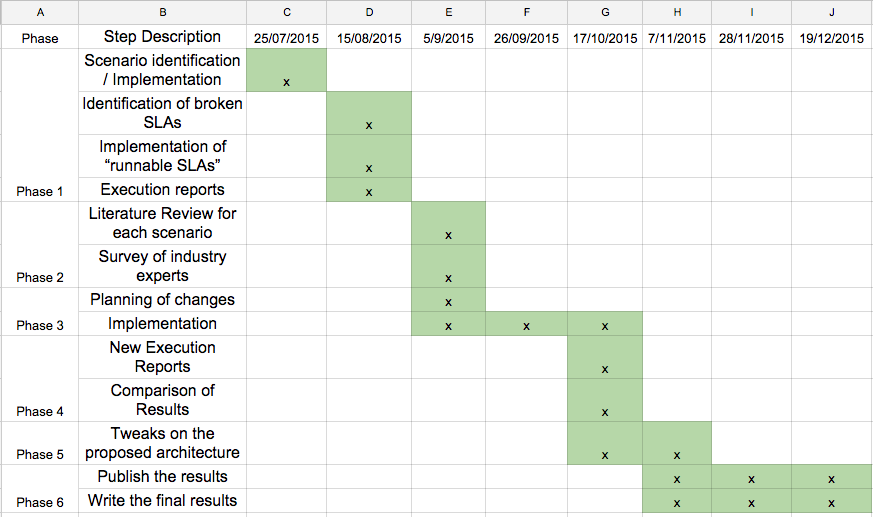
\includegraphics[width=140mm]{schedule.png}
\caption{Schedule.\label{fig:schedule}}
\end{figure}
\end{enumerate}

\end{enumerate}

	
	% Capitulo 3: Terceiro cap�tulo (arquivo Includes/Capitulo3.tex)
	% Cap�tulo 3
\chapter{Proposed solution}

\section{Proposed solution}

Service-Oriented Architecture (SOA) suggests that a Software Component can be seen as a set of sub-services. In the context of a Web Application, for example, it is possible to entirely replace a component just by changing the API address that it uses. This scenario of component replacement on cloud-based applications can be seen on (Figure~\ref{fig:apireplacement}).

\begin{figure}[ht!]
\centering
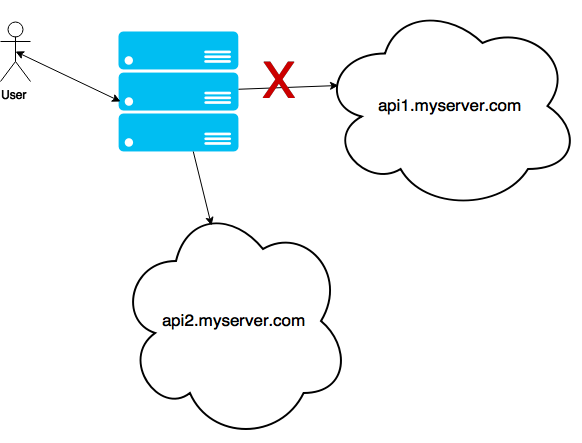
\includegraphics[width=100mm]{api.png}
\caption{Component replacement on cloud-based software.\label{fig:apireplacement}}
\end{figure}

As Section \ref{bibreview} presents, contributions can be made in the context of proposing SLA-Based and user-centered solutions to monitor component replacement scenarios.

In this work we assess the use of a SLA-Guided process to support the migration/replacement of relational databases with NoSQL ones. This process was developed and assessed with case studies.

The boundaries of this work could then be broadened to support the conception of a SLA-Guided process to support the migration/replacement of sotware components based on the cloud in future works.


\section{Roadmap}
%Detalhar l� em cima o que � PDCA
%nosso estudo vai ser baseado no PDCA, detalhado l� em cima, e pode ser dividido em 6 fases principais: 

To provide a better understanding of our work, we splitted the research in six main phases:

\begin{table}[!htb]
   \textsf{\caption{Work Phases.}} \label{tab:WorkPhasesTable}
   \centering
   \medskip
      \begin{tabular}{ | p{1cm}| p{2.5cm} | p {8cm} |}
   \hline
   Phase & Title & Description  \\ \hline
   1 & Identification of Case Studies \& SLAs  & On this step we aim to identify examples where a Database transition is needed or recommended in order to satisfy a SLA.
   We will try to work on production-ready and open-source softwares. If the complexity of these projects is too large for our scope, we will design and develop our own scenarios. \\ \hline
   2 & Plan & After the scenarios have been identified, we will propose architectural changes that could satisfy the SLA. These changes will be proposed by literature reviews and survey of industry experts.\\ \hline
   3 & Do & On this step we implement the architecture proposed on the previous step. \\ \hline
   4 & Check & On the check step we will verify if the proposed architecture and implementation satisfies the SLAs identified on the first step. \\ \hline
   5 & Act & Tweaks can be needed on the proposed architecture and implementation if the SLA is still not satisfied by the changes made on the previous step. On the act phase we investigate what else can be done to satisfy the SLA and refine the process defined on step 2. \\ \hline
   6 & Final Results & On the final step we aim to publish the results of our work on relevant database-related conferences and workshops. \\ \hline
   
   \end{tabular}
\end{table}





Each of these phases is composed by a number of steps, described below:
\begin{enumerate}
\item{Phase 1 - Identification of Case Studies \& SLAs }
\begin{enumerate}
\item {Step 1.1 - Scenario identification / Implementation: On this step we will search for open source projects and real-world scenarios where a Relational Database bottleneck has been identified. If the scope of these scenarios become too large, we will implement our own scenarios; }
\item {Step 1.2 - Identification of broken SLAs: We need to identify that the a set a constraints (i.e: execution time of a query) is not being met by the current architecture;}
\item {Step 1.3 - Implementation of ``runnable SLAs'' : On this step we will implement executable versions of the SLA identified on the previous step. These ``runnable SLAs" will be used to verify that a set of constraints is not being met by the current architecture. }
\item {Step 1.4 - Execution reports: After an executable SLA has been identified and implemented, execution reports will be consolidated to prove that the constraints of the SLA are being broken by the current architecture of the scenario.}

\end{enumerate}


\item{Phase 2 - Plan}
\begin{enumerate}
\item{Step 2.1 - Literature Review for each scenario: We will evaluate and search for solutions on how each scenario can make use of a NoSQL Database to meet the desired SLA; }
\item{Step 2.2 - Survey of industry experts: We will survey industry experts on how they would propose a NoSQL architecture to solve the problem described on each scenario. }
\end{enumerate}

\item{Phase 3 - Do}
\begin{enumerate}
\item{Step 3.1 - Planning of changes: We will gather the results from the previous phase and design the changes that will be performed on each scenario;}
\item{Step 3.2 - Implementation: We will implement the changes identified on the previous step. }
\end{enumerate}

\item{Phase 4 - Check}
\begin{enumerate}
\item {Step 4.1 - New Execution Reports: The same SLAs identified on the first step will be run on the modified scenarios, and execution reports will be consolidated.}
\item {Step 4.2 - Comparison of Results: The reports extracted on steps 4.1 and 1.4 will be compared to check if the changes made on Phase 3 satisfied the proposed SLA.}
\end{enumerate}

\item{Phase 5 - Act}
\begin{enumerate}
\item{Step 5.1 - Tweaks on the proposed architecture: If the SLA isn't being met yet, new changes might be needed, and on this step we join together the phases 2, 3 and 4 to iterate over the needed changes. }
\end{enumerate}


\item{Phase 6 - Final Results}
\begin{enumerate}
\item{Step 6.1 - Publish the results: We will submit the results of this study to academical conferences to have feedback from the community. }
\item{Step 6.2 - Write the final results: All the documents produced by our study and a final dissertation will be sent to the Universidade Federal do Rio Grande do Norte (UFRN).}


\section{Schedule}

A detailed view of the execution flow of our steps can be seen on Figure~\ref{fig:schedule}. 
\begin{figure}[ht!]
\centering
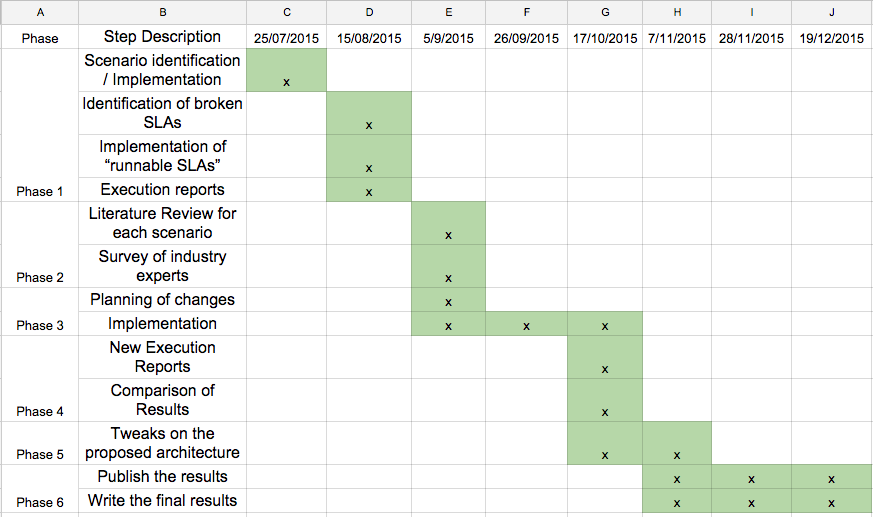
\includegraphics[width=140mm]{schedule.png}
\caption{Schedule.\label{fig:schedule}}
\end{figure}
\end{enumerate}

\end{enumerate}

	
	% Capitulo 4: Quarto cap�tulo (arquivo Includes/Capitulo4.tex)
	% Cap�tulo 4
\chapter{Conclusions}\label{conclusionsChap}

% > E os testes, devo apresentar isso nos guidelines? 

% E a vantagem de ter o Score, mostrando os posts mais relevantes primeiro? 

% > Discuss new app requirements - what elasticsearch enables - Word Cloud, Main integration?

% > E outros tipos de m�tricas, al�m do tempo? 

% Even Gmail, an application that is widely used by hundreds of millions of users, may present errors and unresponsive requests when the workload is too big. After adding a single tag to all emails of an account with over 50.000 emails, for example, the user inbox can become unavailable for some moments, as image \ref{fig:gmailDown} suggests. 

% \begin{figure}[ht!]
% \centering
% 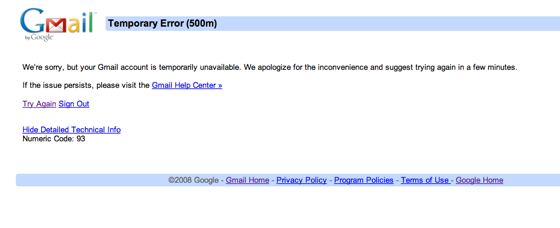
\includegraphics[width=120mm]{Imagens/gmailDown.png}
% \caption{Add a single tag on all Gmail emails.\label{fig:gmailDown}}
% \end{figure}

% Dizer aqui que depois o MySQL lancou a versao com FTS. 
% Dizer que o ES abre um mundo de oportunidades para analytics.

% Dizer que uma das ameacas pode ser o fator de chegada das requests nos cenarios avaliados, que podem nao representar o real. 

% Dizer que dava pra ao inves de tempo os slas serem orientados a acuracia tambem. Dizer de um caso: imagine uma aplicacao que diz quantos pontos tem dentro de um poligono. Com o banco tal a acuracia eh de X. Com o banco Y a acuracia eh de Z.

% TODO: Fix References: https://www.evernote.com/l/AD9tKczyJiBK9KJkJ-s1eNh-AxhMlqz3SXA

% The boundaries of this work could then be broadened to support the conception of a SLA-Guided process to support the migration/replacement of sotware components based on the cloud in future works.
% Dizer tambem que o pessoal recomenda migrar pedacos de feature a feature, como nesse case do Coursera. https://tech.coursera.org/blog/2014/09/23/courseras-adoption-of-cassandra/










\section{Work Phases - TODO: Continue from here}

To provide a better understanding of our work, we splitted the research in six main phases:

\begin{table}[!htb]
   \textsf{\caption{Work Phases.}} \label{tab:WorkPhasesTable}
   \centering
   \medskip
      \begin{tabular}{ | p{1cm}| p{2.5cm} | p {10cm} |}
   \hline
   Phase & Title & Description  \\ \hline
   1 & Identification of Case Studies \& SLAs  & On this step we aim to identify examples where a Database transition is needed or recommended in order to satisfy a SLA.
   We will try to work on production-ready and open-source softwares. If the complexity of these projects is too large for our scope, we will design and develop our own scenarios. \\ \hline
   2 & Plan & After the scenarios have been identified, we will propose architectural changes that could satisfy the SLA. These changes will be proposed by literature reviews and survey of industry experts.\\ \hline
   3 & Do & On this step we implement the architecture proposed on the previous step. \\ \hline
   4 & Check & On the check step we will verify if the proposed architecture and implementation satisfies the SLAs identified on the first step. \\ \hline
   5 & Act & Tweaks can be needed on the proposed architecture and implementation if the SLA is still not satisfied by the changes made on the previous step. On the act phase we investigate what else can be done to satisfy the SLA and refine the process defined on step 2. \\ \hline
   6 & Final Results & On the final step we aim to publish the results of our work on relevant database-related conferences and workshops. \\ \hline
   
   \end{tabular}
\end{table}





% Each of these phases is composed by a number of steps, described below:
% \begin{enumerate}
% \item{Phase 1 - Identification of Case Studies \& SLAs }
%    \begin{enumerate}
%    \item {Step 1.1 - Scenario identification / Implementation: On this step we will search for open source projects and real-world scenarios where a Relational Database bottleneck has been identified. If the scope of these scenarios become too large, we will implement our own scenarios; }
%    \item {Step 1.2 - Identification of broken SLAs: We need to identify that the a set a constraints (i.e: execution time of a query) is not being met by the current architecture;}
%    \item {Step 1.3 - Implementation of ``runnable SLAs'' : On this step we will implement executable versions of the SLA identified on the previous step. These ``runnable SLAs" will be used to verify that a set of constraints is not being met by the current architecture. }
%    \item {Step 1.4 - Execution reports: After an executable SLA has been identified and implemented, execution reports will be consolidated to prove that the constraints of the SLA are being broken by the current architecture of the scenario.}

%    \end{enumerate}


% \item{Phase 2 - Plan}
%    \begin{enumerate}
%    \item{Step 2.1 - Literature Review for each scenario: We will evaluate and search for solutions on how each scenario can make use of a NoSQL Database to meet the desired SLA; }
%    \item{Step 2.2 - Survey of industry experts: We will survey industry experts on how they would propose a NoSQL architecture to solve the problem described on each scenario. }
%    \end{enumerate}

% \item{Phase 3 - Do}
%    \begin{enumerate}
%    \item{Step 3.1 - Planning of changes: We will gather the results from the previous phase and design the changes that will be performed on each scenario;}
%    \item{Step 3.2 - Implementation: We will implement the changes identified on the previous step. }
%    \end{enumerate}

% \item{Phase 4 - Check}
%    \begin{enumerate}
%    \item {Step 4.1 - New Execution Reports: The same SLAs identified on the first step will be run on the modified scenarios, and execution reports will be consolidated.}
%    \item {Step 4.2 - Comparison of Results: The reports extracted on steps 4.1 and 1.4 will be compared to check if the changes made on Phase 3 satisfied the proposed SLA.}
%    \end{enumerate}

% \item{Phase 5 - Act}
%    \begin{enumerate}
%    \item{Step 5.1 - Tweaks on the proposed architecture: If the SLA isn't being met yet, new changes might be needed, and on this step we join together the phases 2, 3 and 4 to iterate over the needed changes. }
%    \end{enumerate}


% \item{Phase 6 - Final Results}
%    \begin{enumerate}
%    \item{Step 6.1 - Publish the results: We will submit the results of this study to academical conferences to have feedback from the community. }
%    \item{Step 6.2 - Write the final results: All the documents produced by our study and a final dissertation will be sent to the Universidade Federal do Rio Grande do Norte (UFRN).}
%    \end{enumerate}

% \section{Schedule}

% A detailed view of the execution flow of our steps can be seen on Figure~\ref{fig:schedule}. 
% \begin{figure}[ht!]
% \centering
% 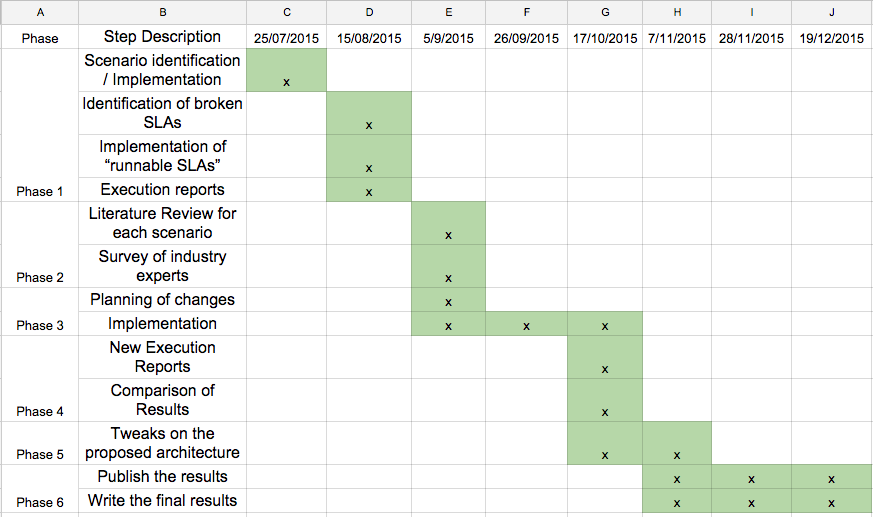
\includegraphics[width=140mm]{schedule.png}
% \caption{Schedule.\label{fig:schedule}}
% \end{figure}
% \end{enumerate}
	
	% Capitulo 5: Quinto cap�tulo (arquivo Includes/Capitulo5.tex)
	% % Cap�tulo 5
\chapter{Cap�tulo 5}

\section{Se��o 1}

Se��o 1


\section{Se��o 2}

Alguns exemplos de cita��o: 

Na tese de Doutorado de Paquete \cite{PaquetePhD}, discute-se sobre algoritmos de busca local estoc�sticos aplicados a problemas de Otimiza��o Combinat�ria considerando m�ltiplos objetivos. Por sua vez, o trabalho de \cite{KnowlesBoundedLebesgue}, publicado nos anais do IEEE CEC de 2003, mostra uma t�cnica de arquivamento tamb�m empregada no desenvolvimento de algoritmos evolucion�rios multi-objetivo, trabalho esse posteriormente estendido para um cap�tulo de livro dos mesmos autores \cite{KnowlesBoundedPareto}. Por fim, no relat�rio t�cnico de \citeonline{Jaszkiewicz}, fala-se sobre um algoritmo gen�tico h�brido para problemas multi-crit�rio, enquanto no artigo de jornal de Lopez \textit{et al.} \cite{LopezPaqueteStu} trata-se do \textit{trade-off} entre algoritmos gen�ticos e metodologias de busca local, tamb�m aplicados no contexto multi-crit�rio e relacionado de alguma forma ao trabalho de Jaszkiewicz (\citeyear{Jaszkiewicz}).

Outros exemplos relacionados encontram-se em \cite{Silberschatz} (livro), \cite{DB2XML} (refer�ncia da Web) e \cite{Angelo} (disserta��o de Mestrado).

\subsection{Subse��o 5.1}

Subse��o 5.1


\subsection{Subse��o 5.2}

Subsection 5.2


\section{Se��o 3}

Se��o 3
		
	% Consideracoes finais
	%% Considera��es finais
\chapter{Considera��es finais}

As considera��es finais formam a parte final (fechamento) do texto, sendo dito de forma resumida (1) o que foi desenvolvido no presente trabalho e quais os resultados do mesmo, (2) o que se p�de concluir ap�s o desenvolvimento bem como as principais contribui��es do trabalho, e (3) perspectivas para o desenvolvimento de trabalhos futuros, como listado nos exemplos de se��o abaixo. O texto referente �s considera��es finais do autor deve salientar a extens�o e os resultados da contribui��o do trabalho e os argumentos utilizados estar baseados em dados comprovados e fundamentados nos resultados e na discuss�o do texto, contendo dedu��es l�gicas correspondentes aos objetivos do trabalho, propostos inicialmente.


\section{Principais contribui��es}

Texto.


\section{Limita��es}

Texto.


\section{Trabalhos futuros}

Texto.
	
	% Bibliografia (arquivo Capitulos/Referencias.bib)
	\bibliography{Capitulos/Referencias}
	\bibliographystyle{abnt-alf}
	
	% Ap�ndice A (arquivo Includes/ApendiceA)
	% Ap�ndice
\apendice
\chapter{Systematic Mapping}
\label{appendix}
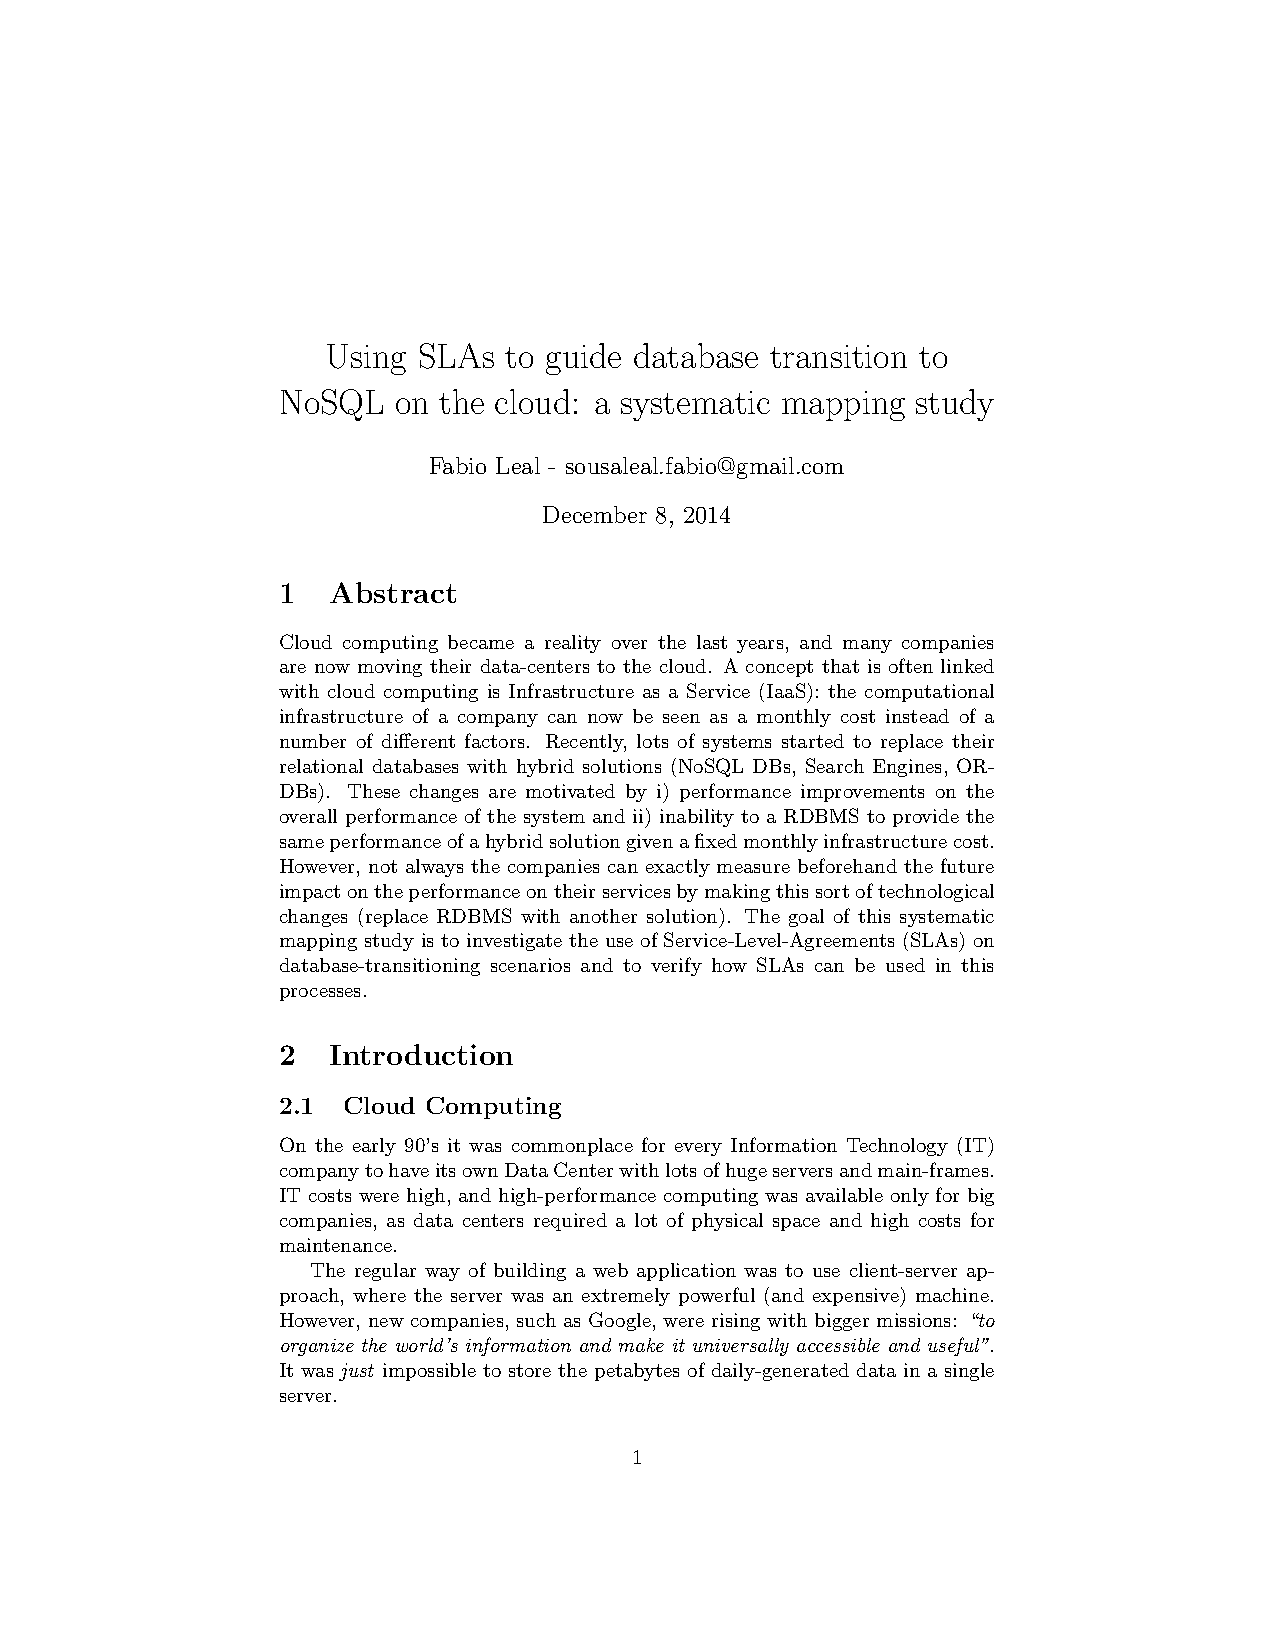
\includepdf[pages=-]{/Users/fabiosl/workspace/ufrn-masters-research/SystematicMapping/submitted/systematicMapping.pdf}
	% Apêndice
\chapter{Execution Reports}
\label{executionreport01}
	% Apêndice
\apendice
\chapter{Execution Reports}
\label{executionreport02}

Execution Report 02 - Time in Millis
\begin{lstlisting}
SIZE=3 SIZE=30 SIZE=300 SIZE=3000 SIZE=30000 SIZE=300000 SIZE=3000000
3	1	2	2	2	2	41
8	1	2	2	2	2	48
1	2	2	2	3	2	30
3	2	2	3	3	2	41
1	2	3	3	1	3	31
4	2	3	2	2	7	34
1	3	3	3	3	2	37
1	2	2	2	3	2	28
1	2	2	2	2	1	31
2	1	6	2	2	1	33
1	1	2	3	3	3	32
1	1	2	3	2	3	46
1	2	2	3	3	1	33
1	2	2	3	3	4	43
1	1	2	3	2	2	38
1	2	2	2	5	2	35
2	1	3	3	2	2	45
2	1	2	1	2	2	29
1	2	2	3	2	2	23
1	2	2	2	2	2	42
1	2	3	2	3	2	35
2	1	1	2	2	3	38
2	2	2	2	3	3	23
2	1	1	2	2	2	20
1	1	2	2	2	2	34
1	4	2	3	2	2	35
1	2	2	2	3	2	30
1	2	2	2	2	2	28
2	2	2	4	3	2	22
1	2	2	3	2	2	25
\end{lstlisting}
	
	% Anexo A (arquivo Includes/AnexoA)
	%% Anexo
\anexo
\chapter{Primeiro anexo}

Os anexos s�o textos ou documentos n�o elaborado pelo autor, que servem de fundamenta��o, comprova��o e ilustra��o.
	
	% P�gina em branco
	\newpage

\end{document}